\subsection{Non-equilibrium carrier trapping and recombination using Shockley-Read-Hall trap states} \label{sssec:dynamic}


To describe charge becoming trapping into trap states and recombination associated with those states the model uses Shockley-Read-Hall (SRH) theory. A 0D depiction of this SRH recombination and trapping is shown in figure \ref{fig:dos_structure}, the free electron and hole carrier distributions are labeled as n free and p free respectively. The trapped carrier populations are denoted with n trap and p trap , they are depicted with filled red and blue boxes. SRH theory describes the rates at which electrons and holes become captured and escape from the carrier traps. If one considers a single electron trap, the change in population of this trap can be described by four carrier capture and escape rates as depicted in figure \ref{fig:dos_structure}. The rate rec describes the rate at which electrons become captured into the electron trap, $r_{ee}$ is the rate which electrons can escape from the trap back to the free electron population, $r_{hc}$ is the rate at which free holes get trapped and $r_{he}$ is the rate at which holes escape back to the free hole population. Recombination is described by holes becoming captured into electron space slice through our 1D traps. Analogous processes are also defined for the hole traps.



\begin{figure}
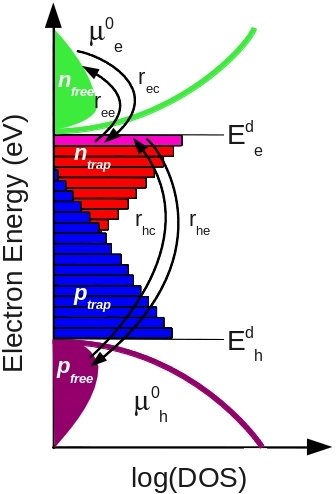
\includegraphics[width=40mm]{./images/dos_structure.jpg}
\caption{Trap filling in both energy and position space as the solar cell is taken from a negative bias
Carrier trapping, de-trapping, and recombination}
\label{fig:dos_structure}
\end{figure}

\begin{table}
\begin{center}
  \begin{tabular}{lll}
  \hline
  Mechanism & Symbol & Description  \\
  \hline
Electron capture rate & $r_{ec}$ & $n v_{th} \sigma_{n} N_{t}(1-f)$ \\
Electron escape rate & $r_{ee}$ & $e_{n} N_{t} f$ \\
Hole capture rate & $r_{hc}$ & $p v_{th} \sigma_{p} N_{t} f$ \\
Hole escape rate & $r_{he}$ & $e_{p} N_{t} (1-f)$\\
  \hline
\end{tabular}
\end{center}
\caption{Shockley-Read-Hall trap capture and emission rates, where $f$ is the fermi-Dirac occupation function and $N_{t}$ is the trap density of a single carrier trap.}
\label{tab:rates}
\end{table}



For each trap level the carrier balance \ref{eq:srhrate} is solved, giving each trap level an independent quasi-Fermi level. Each point in position space can be allocated between 10 and 160 independent trap states.  The rates of each process $r_{ec}$, $r_{ee}$, $r_{hc}$, and $r_{he}$ are give in table \ref{tab:rates}.

\begin{equation}
\label{eq:srhrate}
\frac{\delta n_t}{\partial t}=r_{ec}-r_{ee}-r_{hc}+r_{he}
\end{equation}

The escape probabilities are given by:

\begin{equation}
\label{eq:taile}
e_n=v_{th}\sigma_{n} N_{c} exp \left ( \frac{E_t-E_c}{kT}\right )
\end{equation}

and

\begin{equation}
\label{eq:taile}
e_p=v_{th}\sigma_{p} N_{v} exp \left ( \frac{E_v-E_t}{kT}\right )
\end{equation}

 where $\sigma_{n,p}$ are the trap cross sections, $v_{th}$ is the thermal emission velocity of the carriers, and $N_{c,v}$ are the effective density of states for free electrons or holes.  The distribution of trapped states (DoS) is defined between the mobility edges as

\begin{equation}
\label{eq:taile}
\rho^{e/h}(E)=N^{e/h}exp(E/E_{u}^{e/h})
\end{equation}

where , $N_{e/h}$ is the density of trap states at the LUMO or HOMO band edge
in states/eV and where $E_{U}^{e/h}$ is slope energy of the density of states. 

The value of $N_{t}$ for any given trap level is calculated by averaging the DoS function over the energy ($\Delta E$ ) which a trap occupies:

\begin{equation}
\label{eq:taile}
N_{t}(E)=\frac{\int^{E+\Delta E/2}_{E-\Delta E/2} \rho^{e}{E} dE}{\Delta E}
\end{equation}

The occupation function is given by the equation,
\begin{equation}
f(E_{t},F_{t})=\frac{1}{e^{\frac{E_{t}-F_{t}}{kT}}+1}
\end{equation}
Where, $E_{t}$ is the trap level, and $F_{t}$ is the Fermi-Level of the trap.
The carrier escape rates for electrons and holes are given by



